\documentclass[final,t]{beamer}
\mode<presentation>
{
  \usetheme{I6dv}
}
% additional settings
\setbeamerfont{itemize}{size=\normalsize}
\setbeamerfont{itemize/enumerate body}{size=\normalsize}
\setbeamerfont{itemize/enumerate subbody}{size=\normalsize}

% additional packages
\usepackage{times}
\usepackage{amsmath,amsthm, amssymb, latexsym, bm}
\usepackage{exscale}
\usepackage{booktabs, array}
\usepackage[english]{babel}
\usepackage[latin1]{inputenc}
\usepackage[orientation=landscape,size=custom,width=200,height=120,scale=1.9]{beamerposter}
\listfiles
\graphicspath{{figures/}}

\newcommand*{\LargerCdot}{\raisebox{-0.25ex}{\scalebox{2}{$\cdot$}}}

\title{Automated Flow Cytometry Data Analysis with the OpenCyto Framework}
\author[Ramey et al.]{John Ramey\inst{1}, Greg Finak\inst{1}, Mike Jiang\inst{1}, Jafar Taghiyar\inst{3}, Stephen de Rosa\inst{1,2}, Ryan Brinkman\inst{3}, and Raphael Gottardo\inst{1,2}}
  
\institute[Fred Hutchinson] % (optional, but mostly needed)
{
  \inst{1}%
  Fred Hutchinson Cancer Research Center, Seattle, WA, USA \LargerCdot \ 
  \inst{2}%
  University of Washington, Seattle, WA, USA  \LargerCdot \   
  \inst{3}%
  University of British Columbia, Vancouver, BC, CA
}

% abbreviations
\usepackage{xspace}
\makeatletter
\DeclareRobustCommand\onedot{\futurelet\@let@token\@onedot}
\def\@onedot{\ifx\@let@token.\else.\null\fi\xspace}
\def\eg{{e.g}\onedot} \def\Eg{{E.g}\onedot}
\def\ie{{i.e}\onedot} \def\Ie{{I.e}\onedot}
\def\cf{{c.f}\onedot} \def\Cf{{C.f}\onedot}
\def\etc{{etc}\onedot}
\def\vs{{vs}\onedot}
\def\wrt{w.r.t\onedot}
\def\dof{d.o.f\onedot}
\def\etal{{et al}\onedot}
\makeatother

%%%%%%%%%%%%%%%%%%%%%%%%%%%%%%%%%%%%%%%%%%%%%%%%%%%%%%%
%%%%%%%%%%%%%%%%%%%%%%%%%%%%%%%%%%%%%%%%%%%%%%%%%%%%%%%

\begin{document}
\begin{frame}{} 
  \begin{columns}[t]
    \begin{column}{.3\linewidth}

%%%%%%%%%%%%%%%%%%%%%%%%%%%%%%%%%%%%%%%%%%%%%%%%%%%%%%%

  \begin{block}{Introduction}
          
We have developed the OpenCyto framework, a collection of well-integrated open-source R packages that delivers robust, reproducible, and data-driven gating in an automated pipeline that can incorporate expert-elicited and data-driven prior knowledge.
  \end{block}
  
  \begin{block}{Automated versus Manual Gating}
        \vskip-2ex
          \begin{columns}[t]
    \begin{column}{.5\linewidth}
    \begin{itemize}
      \item \alert{Advantages of Automated Gating}
      \begin{itemize}
        \item Fast and robust
        \item Removes subjectivity
        \item Data-driven
        \item Reproducible
      \end{itemize}
    \end{itemize}
    \end{column}
    \begin{column}{.5\linewidth}
    \begin{itemize}
      \item \alert{Disadvantages of Manual Gating}
      \begin{itemize}
        \item Time-consuming
        \item Inherently subjective
        \vskip0.5ex
        \item Highly variable gate placement from person to person if:
        \begin{itemize}
          \item An experiment is not well-controlled
          \item A marker is not well-resolved
        \end{itemize}
      \end{itemize}
    \end{itemize}
    \end{column}
    \end{columns}
            \vskip2ex
      \end{block}

%%%%%%%%%%%%%%%%%%%%%%%%%%%%%%%%%%%%%%%%%%%%%%%%%%%%%%%
  \begin{block}{The OpenCyto Framework}
  \textcolor{white}{Filler text}\vspace{-4ex}
        \begin{columns}
  \begin{column}{.5\linewidth}
            \begin{itemize}
            \item \alert{Gating Hierarchy}
            \begin{itemize}
      \item Pipeline based on a gating hierarchy defined in a CSV file
      \item Data-derived gates for each sample
      \item Robust gating with Bayesian mixture models via \alert{flowClust 3.0}
      \item Priors are marker-specific, data-driven, and can incorporate expert knowledge
      \item Gating parameters can be optimized to to discriminate between subject cohorts (e.g., vaccination status)
      \item Custom gating algorithms can be utilized via a plugin system
            \end{itemize}
            \end{itemize}
  \vskip2ex
            \centering
            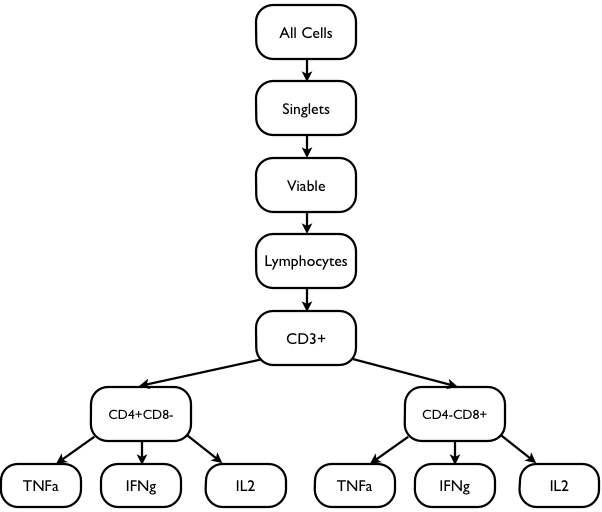
\includegraphics[width=\linewidth]{gating-hierarchy}
          \end{column}
          
          \begin{column}{.5\linewidth}
          \begin{itemize}
            \item \alert{Infrastructure}
          \begin{itemize}
      \item Fast, robust automated gating
      \item Automated pipelines incorporating expert knowledge
      \item Fast processing of large data
      \item C++ libraries and technologies
            \vskip0.25ex
      \begin{itemize}
        \item HDF5
        \item netCDF
        \item boost
      \end{itemize}
            \vskip0.5ex
      \item R Packages
            \vskip0.25ex
      \begin{itemize}
        \item flowWorkspace
        \item flowCore
        \item ncdfFlow
        \item flowClust 3.0
      \end{itemize}
        \end{itemize}
        \end{itemize}
  \vskip5ex
  \centering
            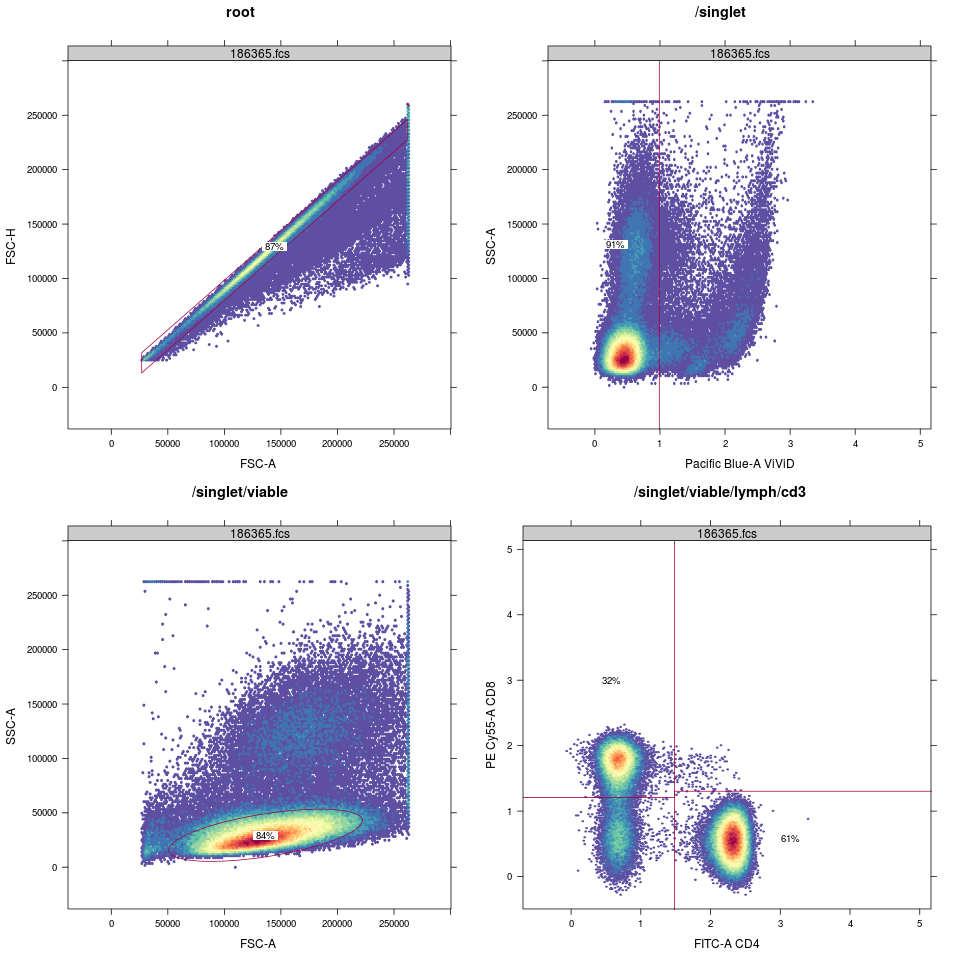
\includegraphics[width=\linewidth]{gates-upstream}
        \end{column}
  \end{columns}



      \end{block}

    \end{column}

%%%%%%%%%%%%%%%%%%%%%%%%%%%%%%%%%%%%%%%%%%%%%%%%%%%%%%%

  \begin{column}{.3\linewidth}
    \begin{block}{Experimental Study -- HVTN 065 Data}
      \begin{itemize}
        \item \alert{Data Description}: 
        \begin{itemize}
          \item ICS data from an HIV Vaccine Trials Network clinical trial
          \item 79 patients -- 67 treated patients and 12 placebos
          \item Time points of interest: 2 (pre-vaccine) and 12 (post-vaccine)
          \item 10 FCS files per patient (5 per time point)
        \end{itemize}

        \vskip-2ex

                \begin{columns}[t]
                  \begin{column}{.1\linewidth}
                  \end{column}
                  \begin{column}{.45\linewidth}
                  \item \alert{Antigens}:
            \begin{itemize}
            \item GAG-1-PTEG
            \item ENV-1-PTEG
            \item Two negative controls
            \item SEB control
          \end{itemize}
                  \end{column}
                  \begin{column}{.45\linewidth}
            \item \alert{Cytokines of Interest}:
          \begin{itemize}
            \item TNF$\alpha$
            \item IFN$\gamma$
            \item IL2
          \end{itemize}
                  \end{column}
              \end{columns}

        \vskip 1ex

        \item \alert{Goals}:
        \begin{itemize}
          \item Automatically gate data using OpenCyto
          \item Extract Boolean subsets of cytokine gates with proportions as features
          \item Classify the vaccination status of the subject cohorts via the elastic net classifier (the {\tt glmnet} R package)
          \item Identify antigen-specific T-cells responding to the vaccine using the markers selected
        \end{itemize}
      \end{itemize}
    \end{block}

%%%%%%%%%%%%%%%%%%%%%%%%%%%%%%%%%%%%%%%%%%%%%%%%%%%%%%%

    \begin{block}{Cytokine Gates -- HVTN065 Data}
      \begin{columns}[t]
                \begin{column}{.45\linewidth}
                        \vskip-35ex
        \begin{itemize}
          \item \alert{Cytokine Gate}:
          \begin{itemize}
            \item Standardize samples across antigens for a patient visit
            \item Construct gate using derivative of kernel density estimate
            \item Gate cut point is selected using a threshold from derivative of pooled densities
            \item Backtransform gate for each stimulation group (antigen)
          \end{itemize}
        \end{itemize}
        \end{column}
        \begin{column}{.55\linewidth}
          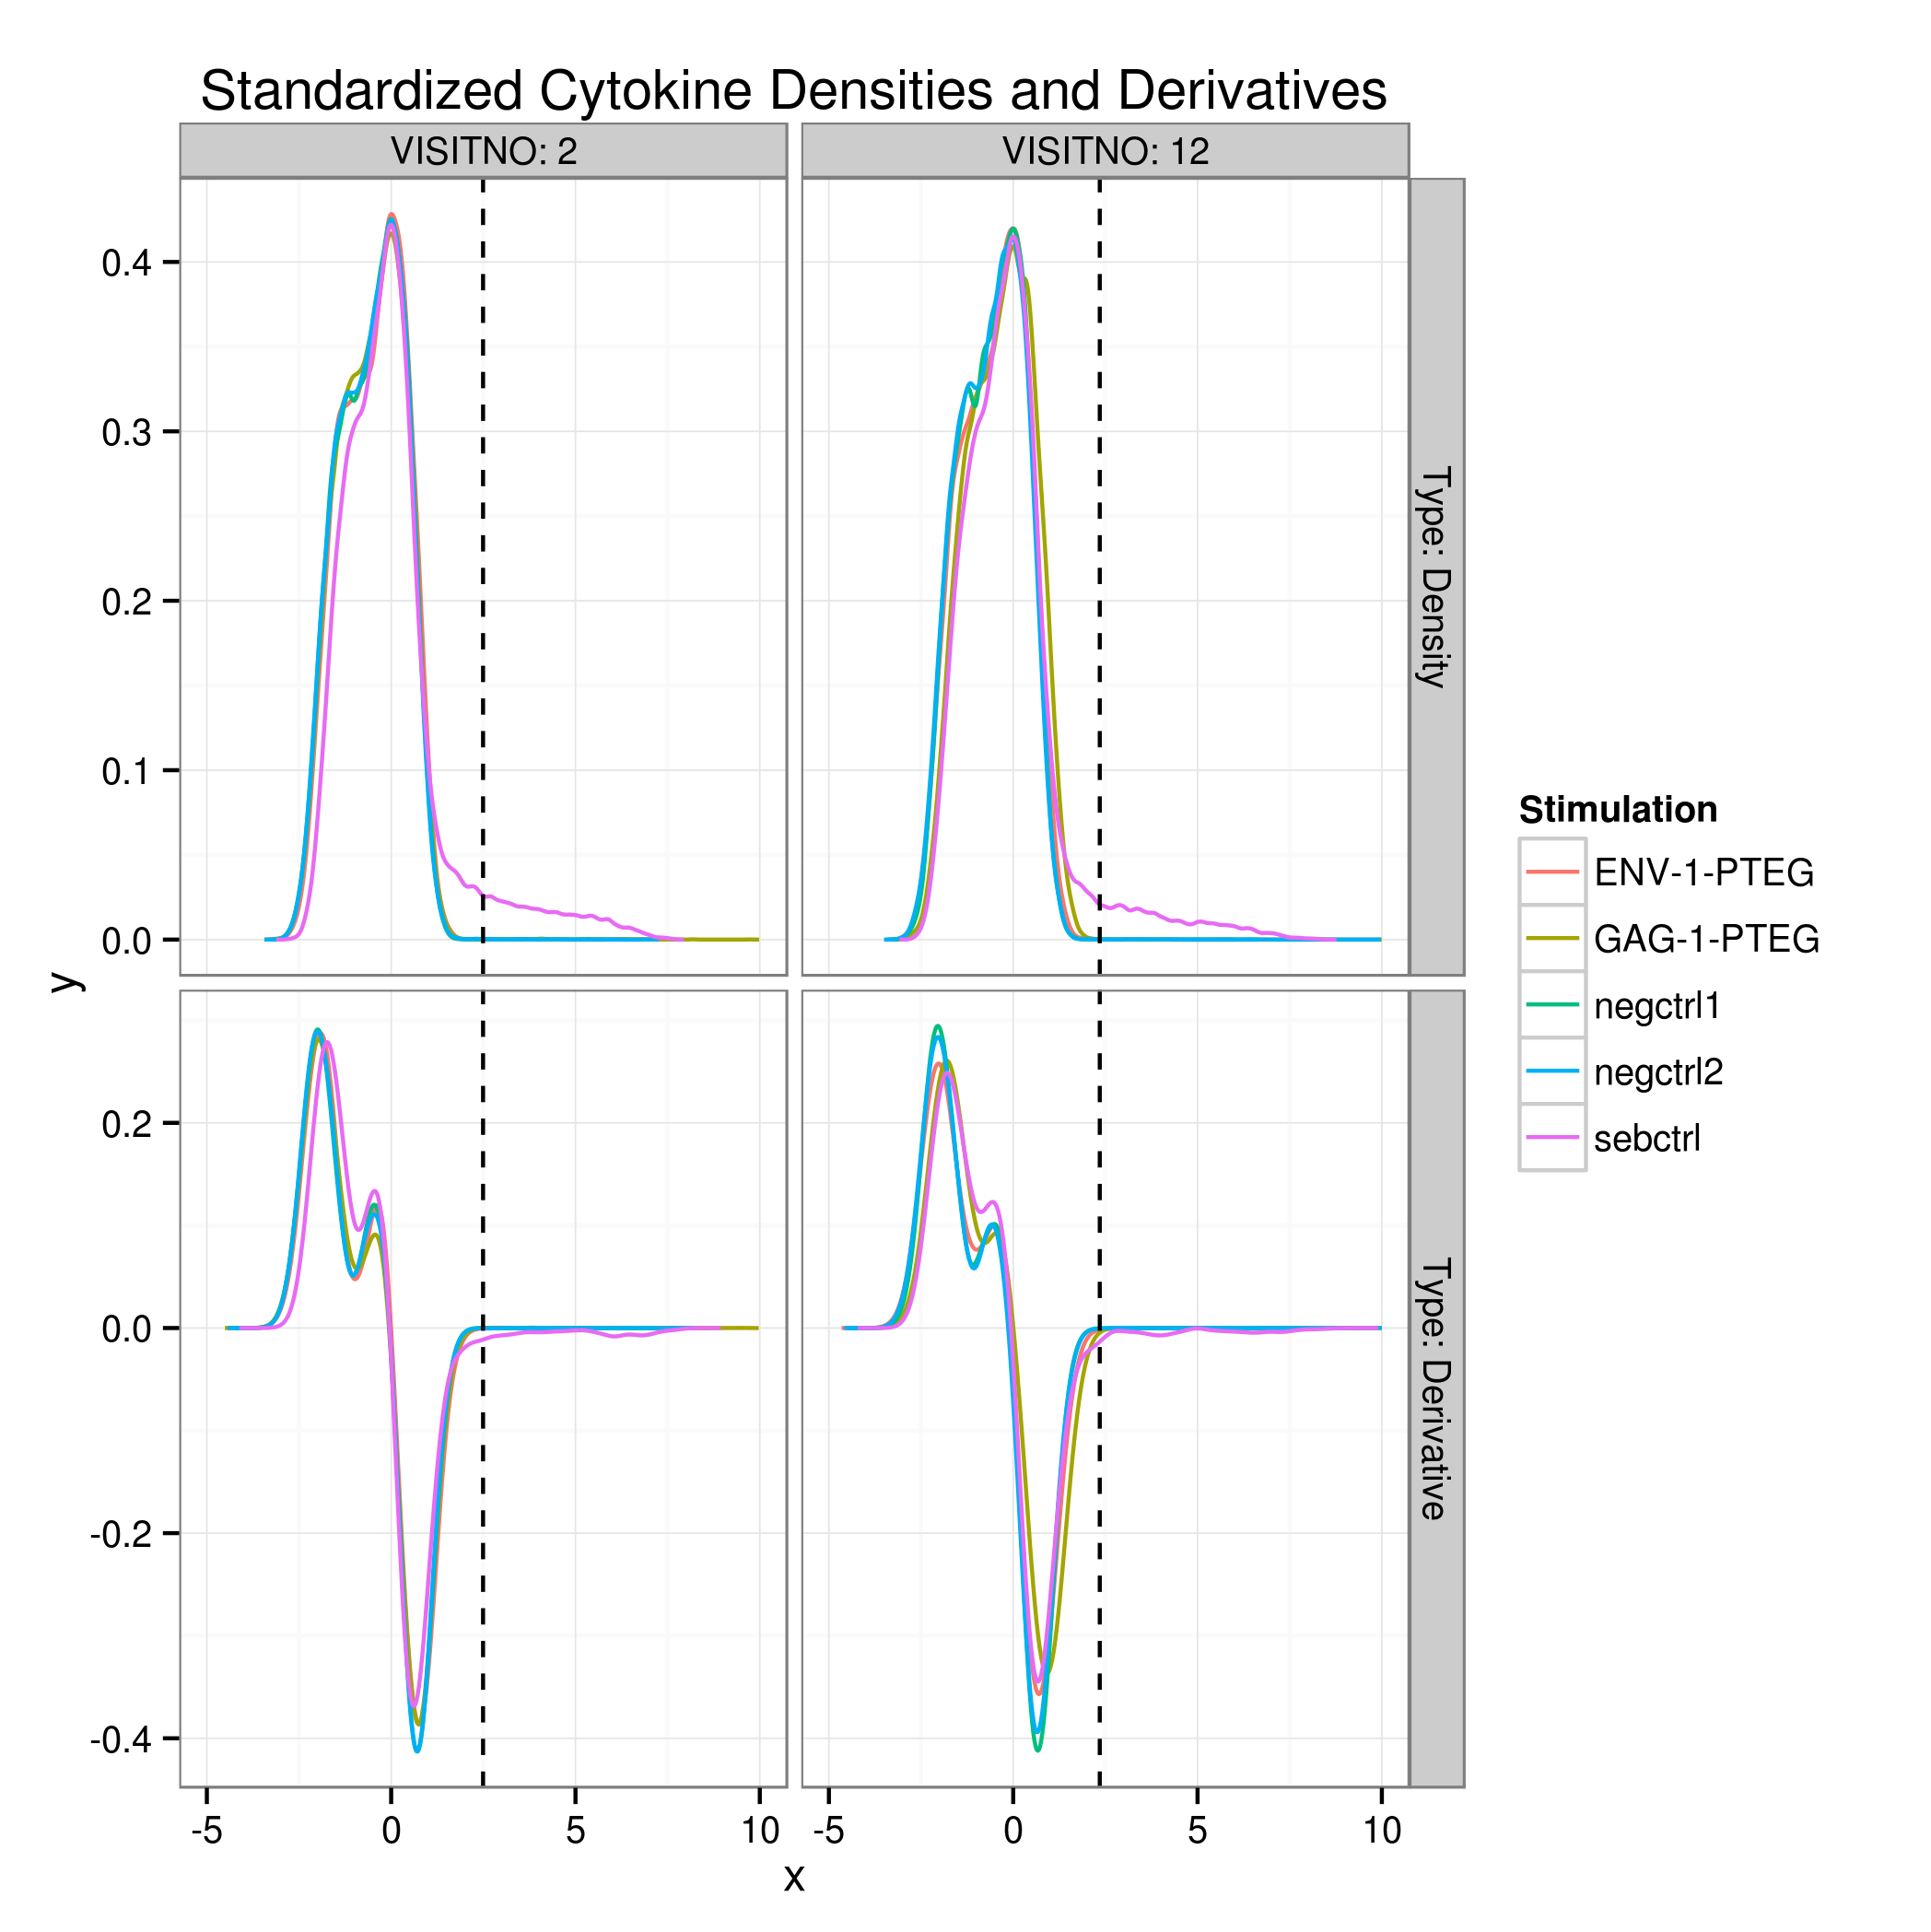
\includegraphics[width=0.95\linewidth]{cytokine-densities-cd4-TNFa}
        \end{column}
      \end{columns}
      \centering
      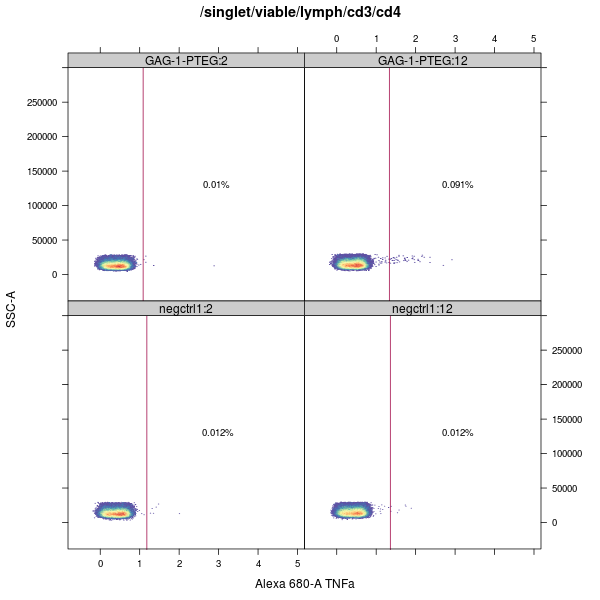
\includegraphics[width=0.44\linewidth]{gates-cd4-TNFa-GAG}
      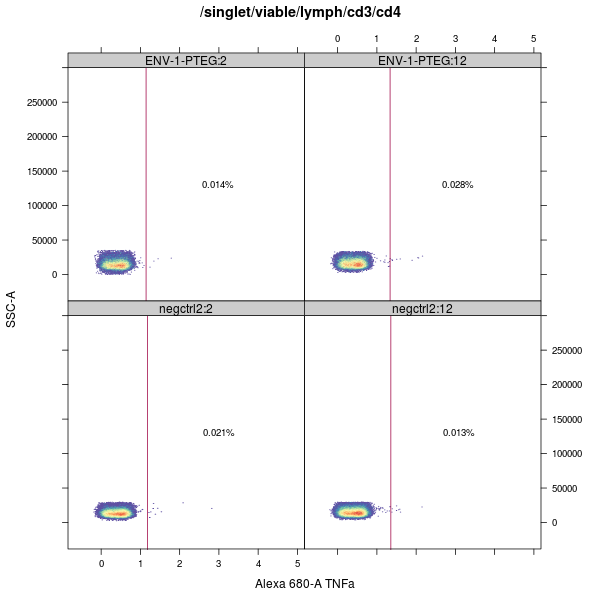
\includegraphics[width=0.44\linewidth]{gates-cd4-TNFa-ENV}
      \vskip-1.5ex
    \end{block}

  \end{column}

%%%%%%%%%%%%%%%%%%%%%%%%%%%%%%%%%%%%%%%%%%%%%%%%%%%%%%%
    
    \begin{column}{.3\linewidth}


%%%%%%%%%%%%%%%%%%%%%%%%%%%%%%%%%%%%%%%%%%%%%%%%%%%%%%%
  \begin{block}{Classification Results -- HVTN065 Data}
        \vskip-2ex
    \begin{columns}[t]
      \begin{column}{.5\linewidth}
      \begin{itemize}
        \item Classifier trained using 60\% of treated patients
        \item Classified remaining 40\% of treated patients as well as placebo patients
        \item Constructed cytokine gates using various tolerance thresholds
        \item Excellent classification performance for smaller tolerance values
        \item GAG-1-PTEG had more discriminatory signal than ENV-1-PTEG
        \item Classification of GAG-1-PTEG placebo patients was no better than random, as expected
      \end{itemize}
      \end{column}
      \begin{column}{.5\linewidth}
        \begin{itemize}
        \item Cytokine Subsets Selected:
        \vskip0.5ex
        \begin{itemize}
          \item \alert{GAG-1-PTEG}:
          \begin{itemize}
            \item CD4/TNFa-IFNg-IL2+
            \item CD4/TNFa+IFNg-IL2+
            \item CD4/TNFa+IFNg+IL2+
          \end{itemize}
          \vskip2ex
          \item \alert{ENV-1-PTEG}:
          \begin{itemize}
            \item CD4/TNFa-IFNg+IL2+
            \item CD4/TNFa+IFNg-IL2-
            \item CD4/TNFa+IFNg-IL2+
            \item CD4/TNFa+IFNg+IL2-
            \item CD4/TNFa+IFNg+IL2+
            \item CD8/TNFa-IFNg+IL2-
            \item CD8/TNFa-IFNg+IL2+
          \end{itemize}
        \end{itemize}
        \end{itemize}
      \end{column}
    \end{columns}
    \vskip2ex
    \centering
    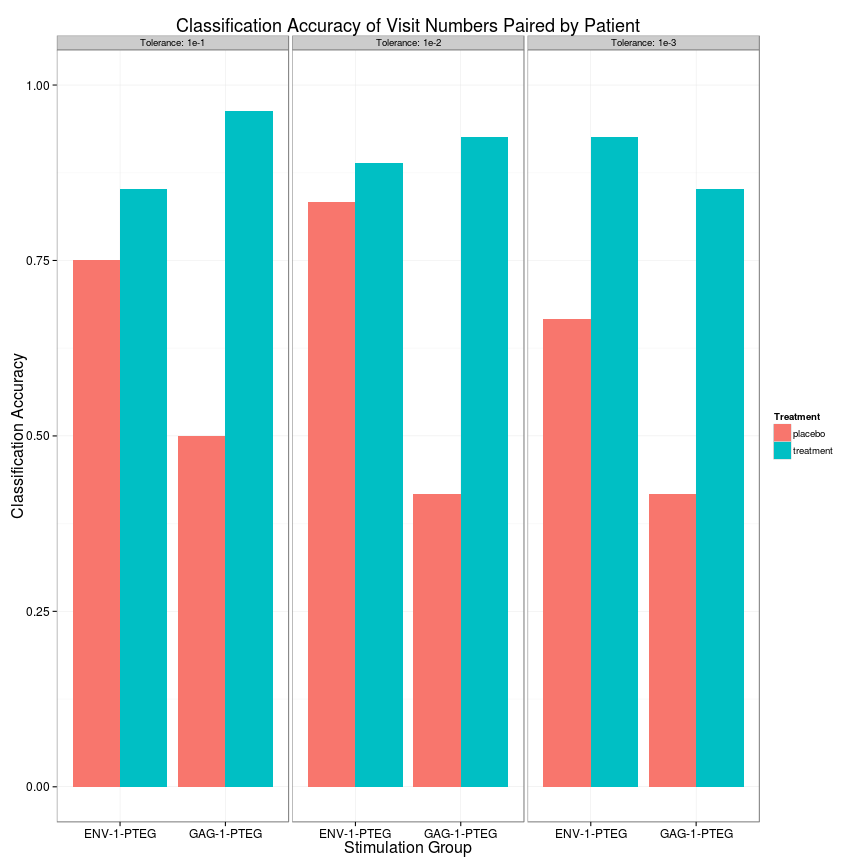
\includegraphics[width=0.5\linewidth]{classification-accuracy-opencyto}
    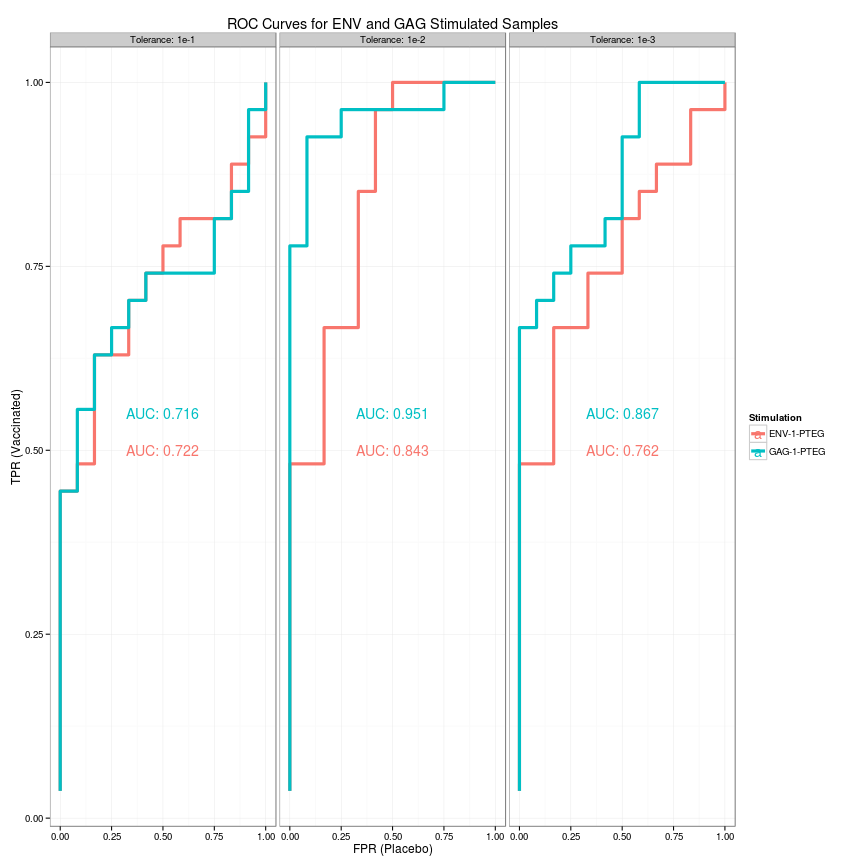
\includegraphics[width=0.5\linewidth]{ROC-opencyto}     
  \end{block}

%%%%%%%%%%%%%%%%%%%%%%%%%%%%%%%%%%%%%%%%%%%%%%%%%%%%%%%                
      \begin{block}{Conclusion}
        \begin{itemize}
            \item OpenCyto:
    \begin{itemize}
    \item Delivers \alert{fast} and \alert{reproducible} automated gating
    \item Attains \alert{robust} gating of rare cell populations
    \item Incorporates \alert{expert} and \alert{data-driven} prior knowledge
    \item Allows optimization of gating parameters to discriminate between subject cohorts based on objective external criteria (e.g., vaccination status)
    \item Enables the researcher to employ \alert{custom} gating algorithms
    \end{itemize}
        \end{itemize}
        \vspace{-1ex}
      \end{block}


%%%%%%%%%%%%%%%%%%%%%%%%%%%%%%%%%%%%%%%%%%%%%%%%%%%%%%%

      \begin{block}{Acknowledgements}
        \vspace{-3ex}
       \begin{columns}[t]
  \begin{column}{.35\linewidth}
          \begin{itemize}
              \item \alert{Funding}
            \begin{itemize}
                \item HIPC
        \item NIH
        \item NIAID
        \item HVTN
            \end{itemize}
    \end{itemize}
  \end{column}
  \begin{column}{.65\linewidth}
          \begin{itemize}
              \item \alert{Codebase}:
            \begin{itemize}
                \item \textbf{\url{http://github.com/RGLab/openCyto}}
            \end{itemize}
    \end{itemize}
  \end{column}
  \end{columns}
      \end{block}
%%%%%%%%%%%%%%%%%%%%%%%%%%%%%%%%%%%%%%%%%%%%%%%%%%%%%%%

    \end{column}
  \end{columns}
\end{frame}

\end{document}

